\let\negmedspace\undefined
\let\negthickspace\undefined
\documentclass[journal]{IEEEtran}
\usepackage[a5paper, margin=10mm, onecolumn]{geometry}
%\usepackage{lmodern} % Ensure lmodern is loaded for pdflatex
\usepackage{tfrupee} % Include tfrupee package

\setlength{\headheight}{1cm} % Set the height of the header box
\setlength{\headsep}{0mm}     % Set the distance between the header box and the top of the text

\usepackage{gvv-book}
\usepackage{gvv}
\usepackage{cite}
\usepackage{amsmath,amssymb,amsfonts,amsthm}
\usepackage{algorithmic}
\usepackage{graphicx}
\usepackage{textcomp}
\usepackage{xcolor}
\usepackage{txfonts}
\usepackage{listings}
\usepackage{enumitem}
\usepackage{mathtools}
\usepackage{gensymb}
\usepackage{comment}
\usepackage[breaklinks=true]{hyperref}
\usepackage{tkz-euclide} 
\usepackage{listings}
% \usepackage{gvv}                                        
\def\inputGnumericTable{}                                 
\usepackage[latin1]{inputenc}                                
\usepackage{color}                                            
\usepackage{array}                                            
\usepackage{longtable}                                       
\usepackage{calc}                                             
\usepackage{multirow}                                         
\usepackage{hhline}                                           
\usepackage{ifthen}                                           
\usepackage{lscape}
\begin{document}

\bibliographystyle{IEEEtran}
\vspace{3cm}

\title{04-10-2023-shift-2(16-30)}
\author{EE24BTECH11055 - Sai Akhila Reddy Turpu}
% \maketitle
% \newpage
% \bigskip
{\let\newpage\relax\maketitle}



\renewcommand{\thefigure}{\theenumi}
\renewcommand{\thetable}{\theenumi}
\setlength{\intextsep}{10pt} % Space between text and floats


\numberwithin{equation}{enumi}
\numberwithin{figure}{enumi}
\renewcommand{\thetable}{\theenumi}

\begin{enumerate}[start = 16]
		


	\item Let a dice be rolled $n$ times. Let the probability of getting odd numbers seven times be equal to the probability of getting odd numbers nine times. If the probability of getting even numbers twice is $\frac{k}{2^{15}}$, then $k$ is equal to
	\begin{enumerate}
	\begin{multicols}{4}
		\item $60$ 
		\item $30$
		\item $90$
		\item $15$
		\end{multicols}
	\end{enumerate}

\item Let a circle of radius $4$ be concentric to the ellipse $15x^2 + 19y^2 = 285.$ Then the common tangents are inclined
to the minor axis of the ellipse at the angle

	
	\begin{enumerate}
	\begin{multicols}{4}
		\item $\frac{\pi}{6}$
		\item $\frac{\pi}{12}$
		\item $\frac{\pi}{3}$
		\item $\frac{\pi}{4}$
	\end{multicols}
	\end{enumerate}
\item Let $\overrightarrow{a} = 2\hat{i} + 7\hat{j} - \hat{k}$, $\overrightarrow{b} = 3\hat{i} + 5\hat{k}$ and $\overrightarrow{c} = \hat{i} + \hat{j} + 2\hat{k}$. Let $\overrightarrow{d}$ be a vector which is perpendicular to both $\overrightarrow{a}$ and $\overrightarrow{b}$, and $\overrightarrow{c}\cdot\overrightarrow{d} = 12$. Then $\brak{-\hat{i} + \hat{j} - \hat{k}}\cdot\brak{\overrightarrow{c}\times\overrightarrow{d}}$is equal to	
	\begin{enumerate}
		\begin{multicols}{4}
		\item $24$
		\item $42$
		\item $48$
		\item $44$
			\end{multicols}
	\end{enumerate}
\item Let $S = \cbrak{z = x + iy : \frac{2z-3i}{4z+2i} \text{is a real number}}.$ Then which of the following is NOT correct?
        
	\begin{enumerate}
		\begin{multicols}{2}
		\item $y \in \brak{-\infty,-\frac{1}{2}} \cup \brak{-\frac{1}{2}, \infty}$
		\item $\brak{x,y} = \brak{0,-\frac{1}{2}}$
		\item $x = 0$
		\item $y + x^2 + y^2 \neq -\frac{1}{4}$
		\end{multicols}
	\end{enumerate}
\item Let the line $\frac{x}{1} = \frac{6-y}{2} =\frac{z+8}{5}$ intersect the lines $\frac{x-5}{4} = \frac{y-7}{3} = \frac{z+2}{1}$ and $\frac{x+3}{6} = \frac{3-y}{3} = \frac{z-6}{1}$ at the points $\vec{A}$ and $\vec{B}$ respectively. Then the distance of the mid-point of the line segment $AB$ from the plane $2x - 2y + z = 14$ is:
	
	\begin{enumerate}
			\begin{multicols}{4}
			\item $3$
			\item $\frac{10}{3}$
			\item $4$
			\item $\frac{11}{3}$
			\end{multicols}
	\end{enumerate}
\item The sum of all four-digit numbers that can be formed using all the digits $2, 1, 2, 3$ is equal to \underline{\hspace{1 cm}}. 
\item In the figure, $\theta_1 + \theta_2 = \frac{\pi}{2}$ and $\sqrt{3}\brak{BE} = 4\brak{AB}$. If the area of $\triangle CAB$ is $2\sqrt{3} - 3 {\text{unit}}^2$, when $\frac{\theta_2}{\theta_1}$ is the largest, then the perimeter of $\triangle CED$ is equal to \underline{\hspace{1 cm}}. 
	\begin{center}
	\begin{tikzpicture}
	%\begin{center}
    % Define coordinates for points
    \coordinate [label=below:$A$] (A) at (0,0);
    \coordinate [label=left:$C$] (C) at (0,2);
    \coordinate [label=below:$B$] (B) at (4,0);
    \coordinate [label=above:$E$] (E) at (4,6);
    \coordinate [label=right:$D$] (D) at (4,2);

    % Draw the triangle CAB
    %\draw [thick] (C) -- (A) -- (B) -- cycle;

    % Draw lines CE and DE
    \draw [thick] (C) -- (E);
    \draw [thick] (E) -- (D);
    \draw [thick] (D) -- (C);
    \draw [thick] (A) -- (C);
    \draw [thick] (A) -- (B);
    \draw [thick] (B) -- (D);
    \draw [thick] (B) -- (C);

    % Label the points
    %\node at (C) {$C$};
    %\node at (A) {$A$};
    %\node at (B) {$B$};
    %\node at (E) {$E$};
    %\node at (D) {$D$};

    % Mark the angles
    \pic [draw, "$\theta_2$", angle eccentricity=1.2] {angle = D--C--E};
    \pic [draw, "$\theta_1$", angle eccentricity=1.2] {angle = C--B--A};
    \tkzMarkRightAngle(E,D,C)
		\tkzMarkRightAngle(C,A,B)
		\tkzMarkRightAngle(D,B,A)
		%\end{center}

\end{tikzpicture}
	\end{center}
\item Let the tangent at any point $\vec{P}$ on a curve passing through the points $\brak{1,1}$ and $\brak{\frac{1}{10},100}$, intersect positive x-axis and y-axis at the points $\vec{A}$ and $\vec{B}$ respectively. If $PA : PB = 1 : k$ and $y=y\brak{x}$ is the solution of the differential equation $e^{\frac{dy}{dx}} = kx + \frac{k}{2}, y\brak{0} = k$, then $4y\brak{1} -\log e^3$ is equal to \underline{\hspace{1 cm}}. 
\item Suppose $a_1, a_2, 2, a_3, a_4$ be in an arithmetico-geometric progression. If the common ratio of the corresponding geometric progression is $2$ and the sum of all $5$ terms of the arithmetico-geometric progression is $\frac{49}{2}$, then $a_4$ is equal to \underline{\hspace{1 cm}}. 
\item If the area of the region $\cbrak{\brak{x,y} : \abs{x^2-2} \le x}$ is $A$, then $6A + 16\sqrt{2}$ is equal to \underline{\hspace{1 cm}}. 
\item Let the foot of perpendicular from the point $\vec{A} \brak{4,3,1}$ on the plane $P : x - y + 2z +3 = 0$ be $\vec{N}$. If $\vec{B}\brak{5,\alpha,\beta}, \alpha, \beta \in \mathbb{Z}$ is a point on plane $P$ such that the area of triangle $ABN$ is $3\sqrt{2}$, then $\alpha^2 + \beta^2 +\alpha\beta $ is equal to \underline{\hspace{1 cm}}. 
\item Let $S$ be the set of values of $\lambda$, for which the system of equations 
\begin{align*}
	6\lambda x - 3y + 3z &= 4\lambda^2,\\ 
	2x + 6\lambda y + 4z &= 1, \\
	3x + 2y + 3\lambda z &= \lambda 
\end{align*}
has no solution. Then $12 \sum_{\lambda \in S} |\lambda|$ is equal to \underline{\hspace{1 cm}}. 
\item If the domain of the function $f\brak{x} = \sec^{-1}\brak{\frac{2x}{5x+3}}$ is $[\alpha,\beta) \cup (\gamma,\delta]$, then $\abs{3\alpha +10\brak{\beta + \gamma} + 21\delta}$ is equal to \underline{\hspace{1 cm}}. 
\item Let the quadratic curve passing through the point $\brak{-1,0}$ and touching the line $y=x$ at $\brak{1,1}$ be $y=f\brak{x}$. Then the x-intercept of the normal to the curve at the point $\brak{\alpha,\alpha + 1}$ in the first quadrant is \underline{\hspace{1 cm}}.
\item Let the equations of two adjacent sides of a parallelogram $ABCD$ be $2x-3y=-23$ and $5x + 4y = 23$. If the equation of one of its diagonal $AC$ is $3x + 7y = 23$ and the distance of $A$ from the other diagonal is $d$, then $50d^2$ is equal to \underline{\hspace{1 cm}}. 
\end{enumerate}
\end{document}
